% ==================================================
% CHAPTER 7: Comparing cosmic muon and x-ray relative strip position offsets %
% ==================================================

\chapter{Comparing cosmic muon and x-ray relative strip position offsets}
\label{chap:comparison}
% Edit count: Lia - 1, Brigitte - 0

The goal of the work presented in this thesis is to validate the local strip position offsets measured with x-ray data with results obtained using cosmic ray data. The challenge was that the x-ray dataset provided absolute local offsets measured in the ATLAS coordinate system while the cosmics dataset provided relative local offsets measured with respect to a reference frame defined by two of four sTGC layers in a quadruplet~-- which could not be compared directly. To address the challenge, the x-ray local offsets were used to calculate relative local offsets. Relative local offsets on each sTGC layer obtained with x-ray and cosmics data calculated using the same two sTGC reference layers are compared for each area where x-ray data is available. The results of the comparison are presented here.

% The x-ray relative local offset is opposite sign to the x-ray residual reconstructed from an abstract track using the beam profile centers on each layer as the track hits. The cosmics relative local offset was inferred from the Gaussian mean of muon track residuals in a \SI{100}{mm} by \SI{100}{mm} area, referred to the as the mean cosmics residual.
% --------------------------------------------------
% \section{Evaluating}
% --------------------------------------------------


%---------------------------------------------------
\section{Results}
%---------------------------------------------------
\label{sec:results}

Relative local offsets have the same value but opposite sign to the mean cosmics and x-ray residuals. For the remainder of this chapter, the means of cosmic track residual distributions will be referred to as mean cosmics residuals. 

Mean cosmics and x-ray residuals on sTGC layer 2 calculated with reference layers 1 and 3 across the quadruplet surface are shown in figure~\ref{fig:res_compare_th2} for sTGC quadruplets QL2.P.11 and QL2.P.8. Figure~\ref{fig:res_compare_th2} is a superposition of figures~\ref{fig:res_mean_th2} and \ref{fig:xray_res_th2}.

\newpage
\thispagestyle{empty}
\newgeometry{top=0.5in,bottom=0.5in}
\begin{figure}
\centering
\begin{subfigure}{\textwidth}
  \centering
  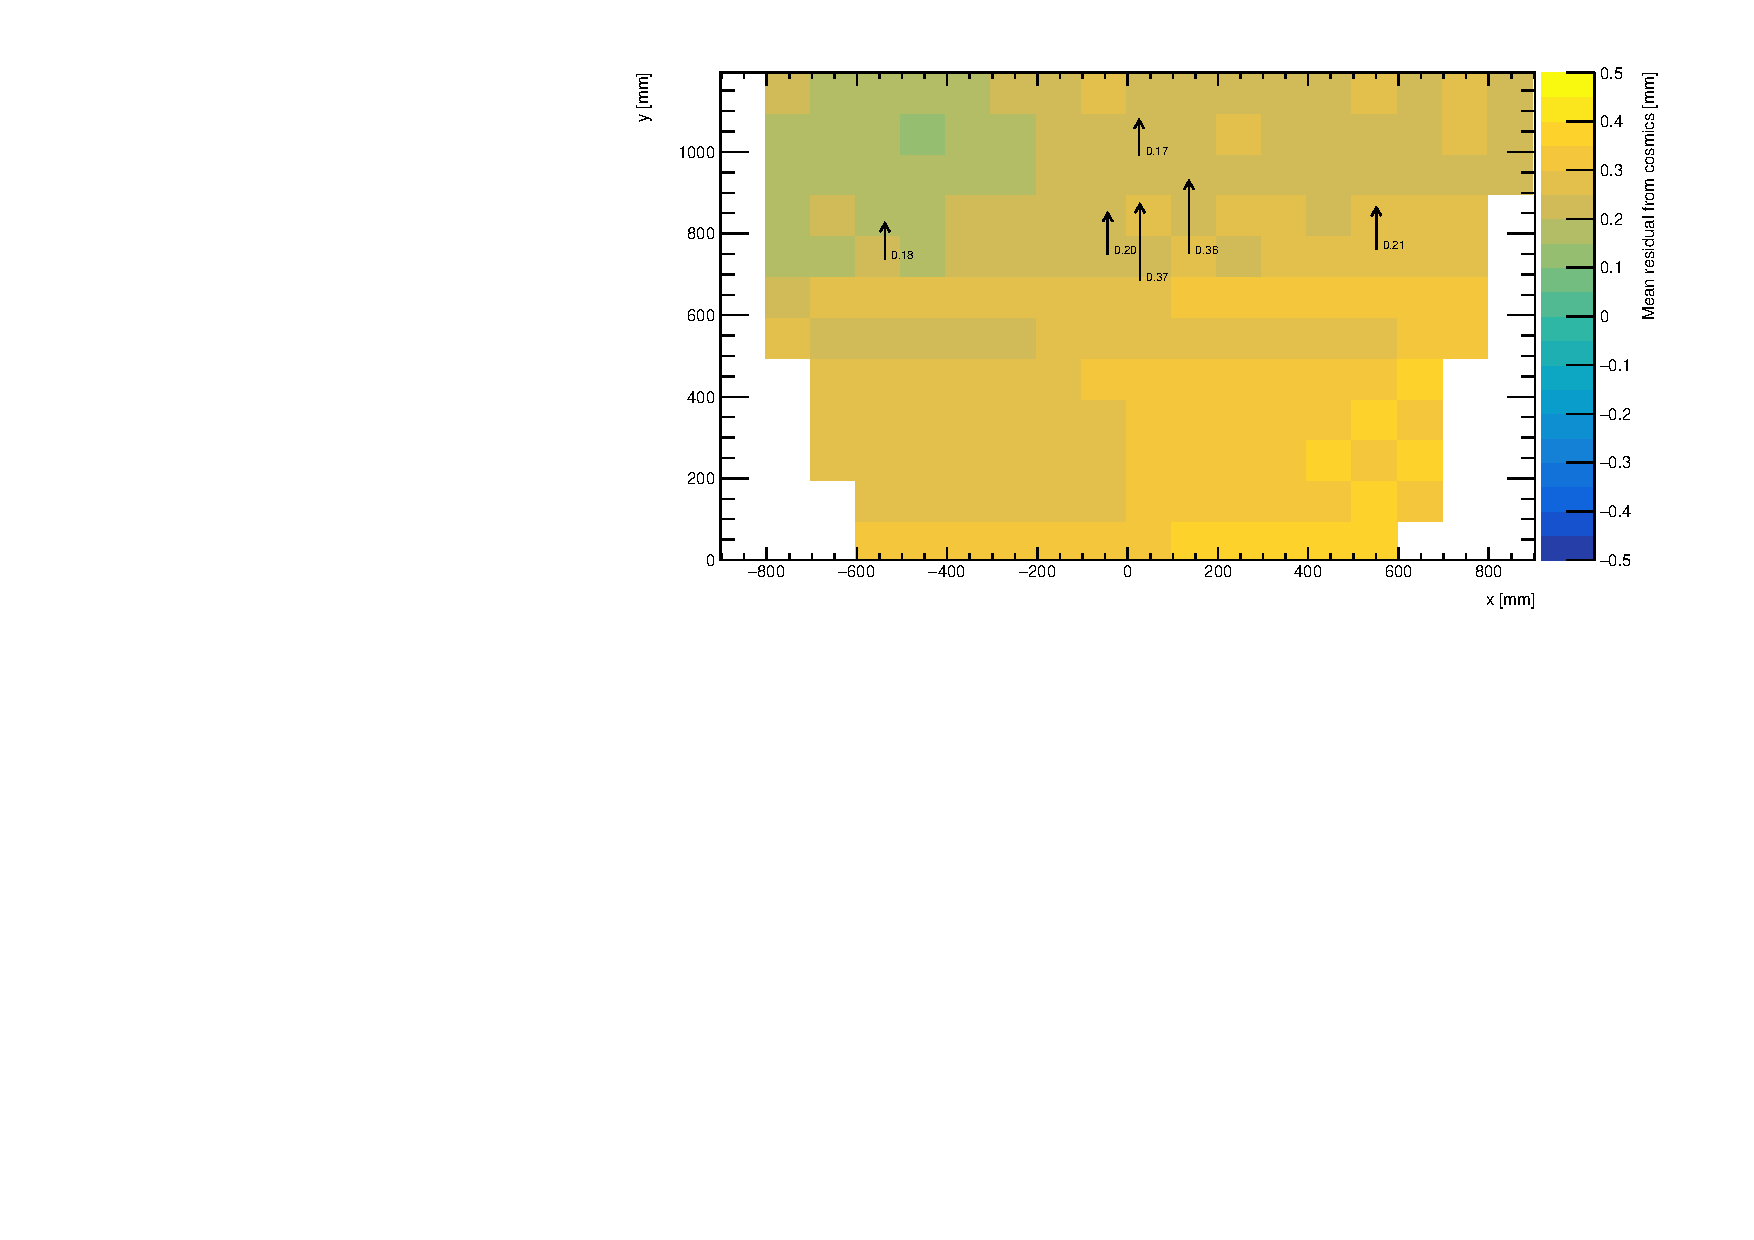
\includegraphics[width=\linewidth]{figures/QL2P11_compare_residuals_th2_layer2_fixedlayers13.pdf}
  \caption{Mean cosmics and x-ray residuals on sTGC layer 2 of quadruplet QL2.P.11 obtained using reference layers 1 and 3.}
  \label{fig:res_compare_th2_ql2p11}
\end{subfigure}%
\vspace*{\floatsep}
\begin{subfigure}{\textwidth}
  \centering
  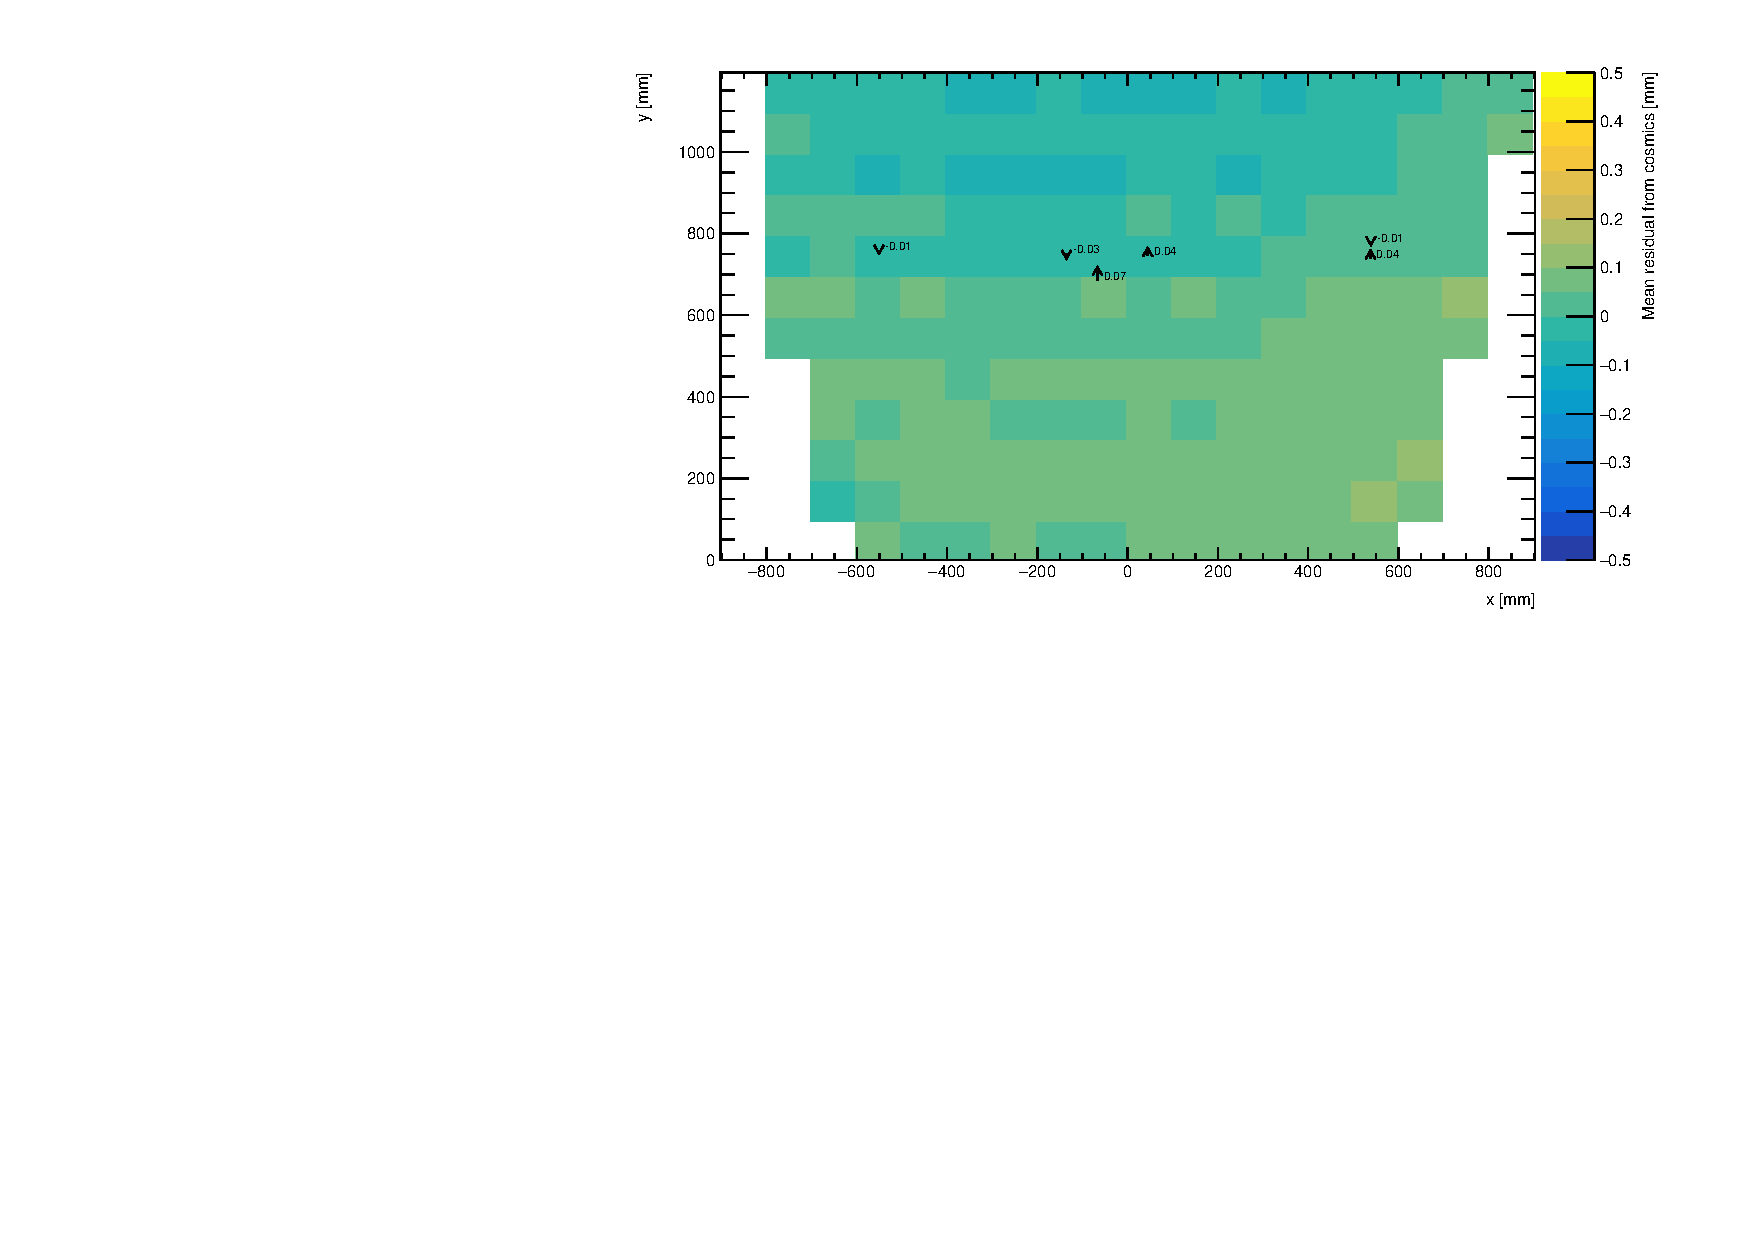
\includegraphics[width=\linewidth]{figures/QL2P08_compare_residuals_th2_layer2_fixedlayers13.pdf}
  \caption{Means cosmics and x-ray residuals on sTGC layer 2 of quadruplet QL2.P.8 obtained using reference layers 1 and 3.}
  \label{fig:res_compare_th2_ql2p8}
\end{subfigure}
\caption{The mean cosmics residuals are shown using colour. The x-ray residuals available at nominal gun positions are drawn as arrows and the value of the residual annotated in millimeters with uncertainty $\pm$\SI{0.15}{mm}. The length of the arrows is 500 times the value of the x-ray residual, scaled for visibility. These plots are a superposition of figures~\ref{fig:res_mean_th2} and \ref{fig:xray_res_th2}.}
\label{fig:res_compare_th2}
\end{figure}
\newpage
\restoregeometry

Figure~\ref{fig:res_compare_th2_ql2p11} shows that for QL2.P.11 the x-ray residuals are of the same sign and order as the mean cosmics residuals, as can be seen by comparing the annotated value of the x-ray residual to the mean cosmics residual represented in the nearest coloured bin. QL2.P.11's mean cosmics and x-ray residuals are correlated. 

For QL2.P.8, figure~\ref{fig:res_compare_th2_ql2p8} shows that the x-ray residuals are of the right order compared to the mean cosmics residuals; however, the value of the x-ray residuals are within their uncertainty so the correlation is not manifest. While the x-ray residuals do not reveal a pattern in the relative local offsets across the layer's surface, the mean cosmics residuals show a structure to the relative local offsets, revealed by how they vary smoothly over the surface of sTGC layer 2. 

The comparison of mean cosmics and x-ray residuals was done for several sTGC quadruplets for all possible tracking combinations. Scatter plots of the x-ray and mean cosmics residuals on QL2.P.11 and QL2.P.8 for all tracking combinations are shown in figures~\ref{fig:correlation} and \ref{fig:no_correlation} and reveal the degree of correlation between the datasets. In these correlation plots, each rectangle is centered on the value of a mean cosmics and x-ray residual pair calculated with a given tracking combination for every x-ray gun position where data is available. The height and width of the rectangles are the uncertainty in the mean cosmics and x-ray residuals respectively. Note that in the scatter plots, the regions of interest where cosmics tracks are included in the calculation of the mean of residuals are exactly centered on the nominal x-ray beam positions, unlike in figure~\ref{fig:res_compare_th2}.

\begin{figure}
    \centering
    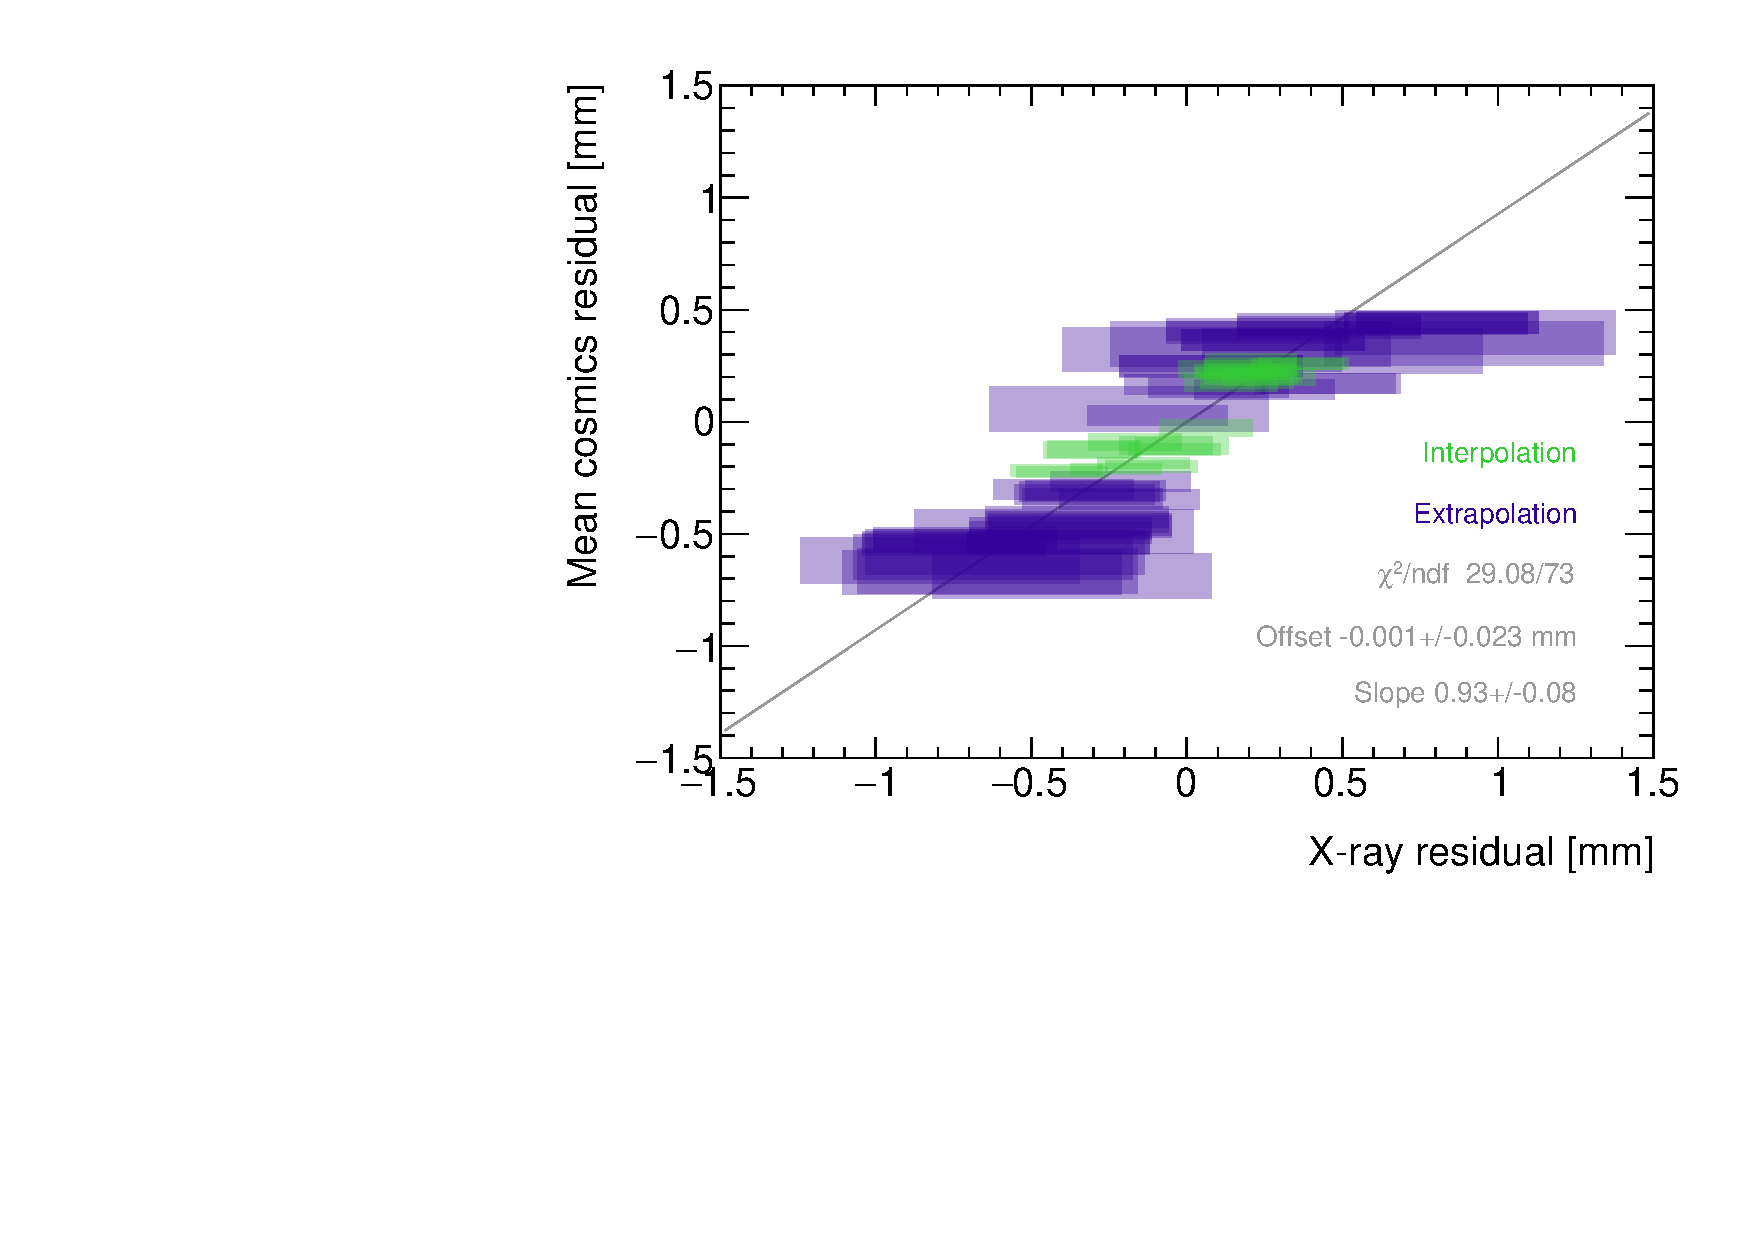
\includegraphics[width = \textwidth]{figures/figure_QL2P11_3100V_2021-08-05_QL2P11_local_cosmic_and_xray_data_correlation_plot.pdf}
    \caption{Correlation plot between x-ray and mean cosmics residuals for all tracking combinations for QL2.P.11. Each rectangle is centered on an x-ray and mean cosmics residual pair calculated at a given x-ray gun position and for a certain tracking combination. The width of the rectangles in $x$ and $y$ are the uncertainty in the x-ray and mean cosmics residual respectively. A printer-friendly version of this plot is available in appendix~\ref{appendix:print}.}
    \label{fig:correlation}
\end{figure}

The fitted slope and offset in figure~\ref{fig:correlation} show that the two QL2.P.11 datasets are correlated. The large uncertainty on the x-ray residuals set a limit on the sensitivity of the analysis, for if the absolute value of the x-ray residuals of a quadruplet were smaller than the x-ray residual uncertainties, no conclusion about the correlation could be drawn, as is the case for layer 2 of sTGC quadruplet QL2.P.8 (figure~\ref{fig:no_correlation}). This result is reflected in the small x-ray residuals shown in figure~\ref{fig:res_compare_th2_ql2p8} that do not reveal a pattern in the relative local offsets across the surface of sTGC layer 2. However, figure~\ref{fig:no_correlation} shows that the x-ray and mean cosmics residuals are clustered approximately around zero as is expected for a quadruplet with small relative misalignments between layers.

\begin{figure}
    \centering
    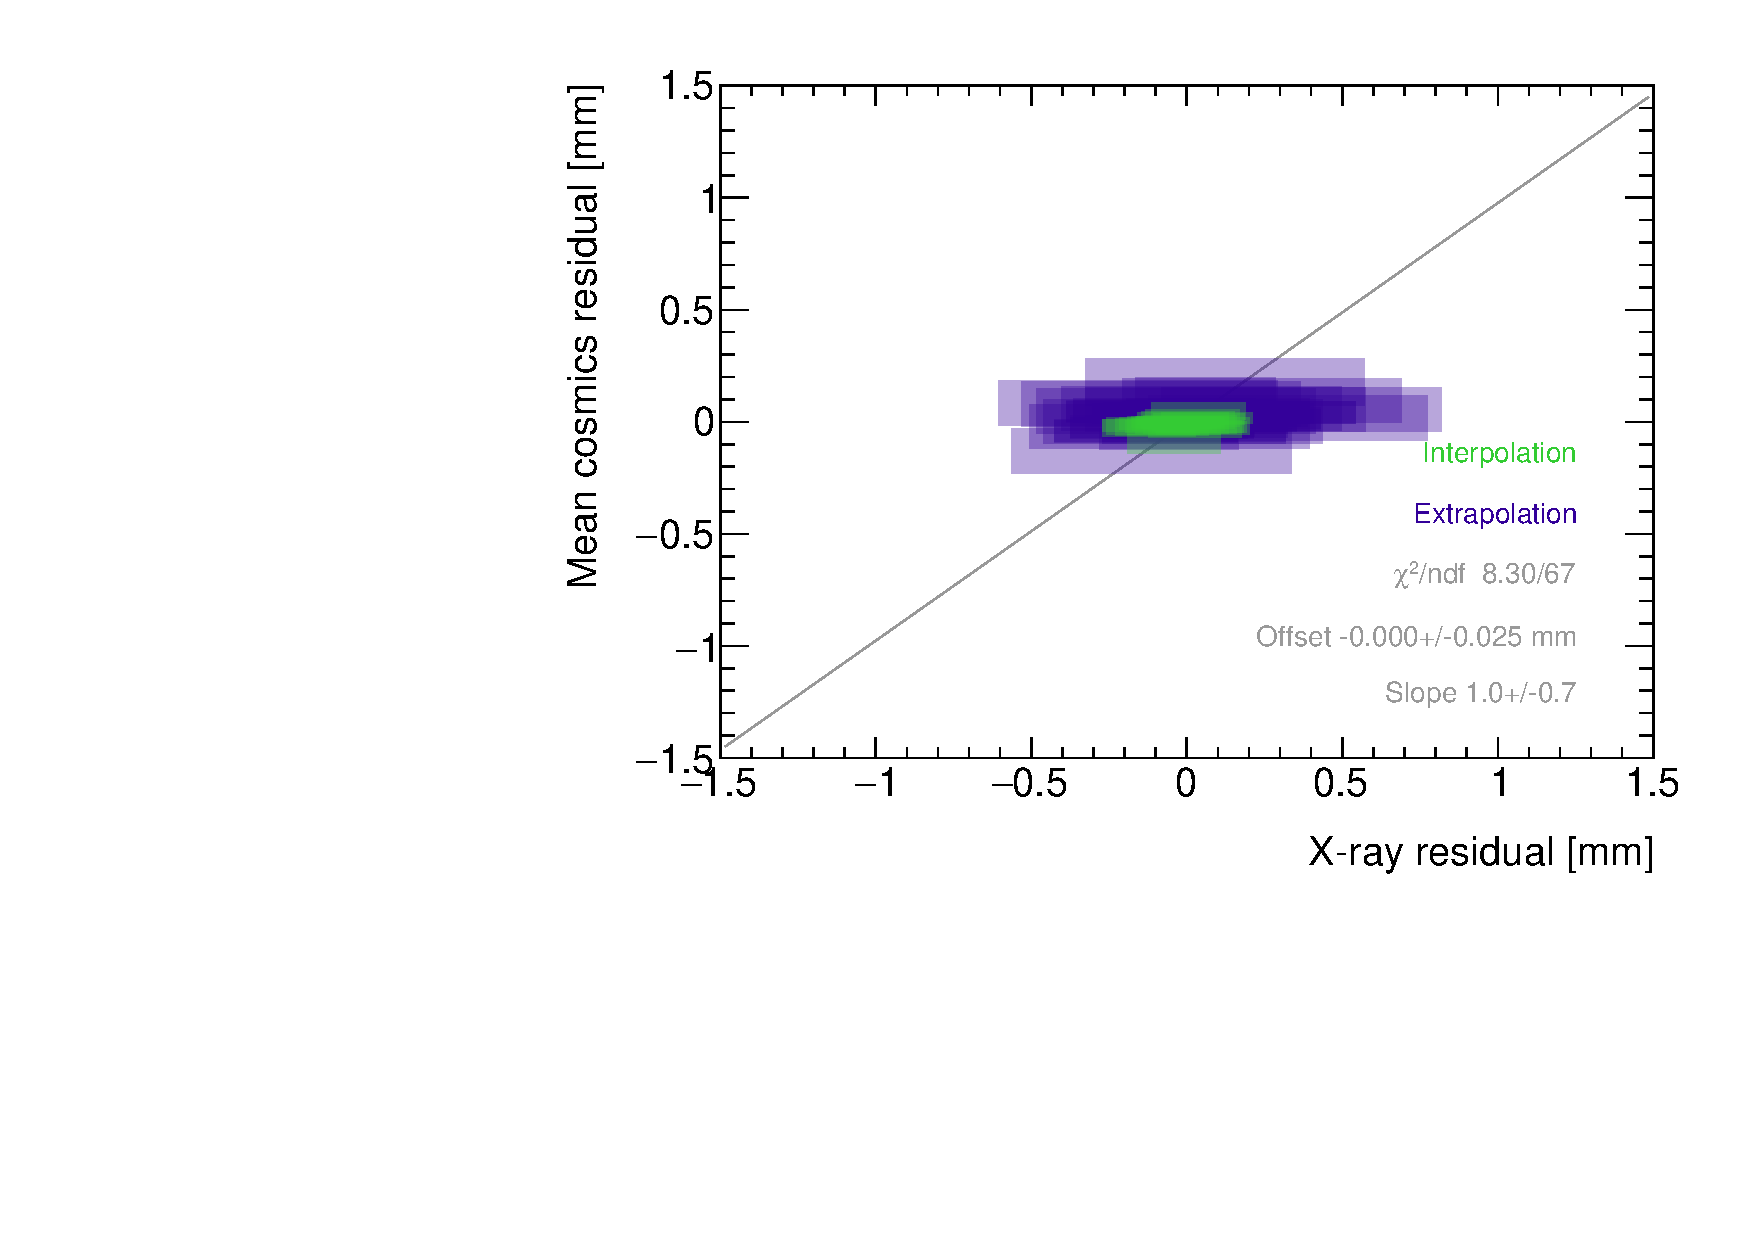
\includegraphics[width = \textwidth]{figures/figure_QL2P08_3100V_2021-08-16_QL2P08_local_cosmic_and_xray_data_correlation_plot.pdf}
    \caption{Correlation plot between x-ray and mean cosmics residuals for all tracking combinations for QL2.P.8. Each rectangle is centered on an x-ray and mean cosmics residual pair calculated at a given x-ray gun position and for a certain tracking combination. The width of the rectangles in $x$ and $y$ are the uncertainty in the x-ray and mean cosmics residuals respectively. A printer-friendly version of this plot is available in appendix~\ref{appendix:print}.}
    \label{fig:no_correlation}
\end{figure}

There are three patterns in the residuals on the scatter plot explained by geometry. First, for both datasets the uncertainty in the extrapolated track residuals were larger than the interpolated track residuals because of the extrapolation lever arm. For the x-ray residuals, the effect of the lever arm on the uncertainty was direct since the residual was calculated from a single straight line; for the mean cosmics residuals it is the widening of the residual distributions due to the extrapolation lever arm that increases the uncertainty in the fitted means of residuals. Second, residuals calculated through extrapolation tend to be larger because the extrapolation lever arm can produce more extreme values of the track position on the layer of interest. Third, the points in figure~\ref{fig:correlation} are geometrically correlated (e.g. they seem to be roughly mirrored around the origin). This is expected since the residuals calculated using a given set of three layers should be geometrically correlated by the local offsets on each layer (the $d_{local, i}$ on each layer as defined in equation~\ref{eqn:local_translation}). 

% --------------------------------------------------
\section{Discussion}
% --------------------------------------------------

Several sTGC quadruplets were tested for each quadruplet construction geometry built in Canada. Each quadruplet fell into one of the two categories: residuals large enough to see a correlation, or residuals too small to see a correlation. Since the x-ray and mean cosmics residuals can be used to calculate relative local offsets between the layer and the two reference layers, quadruplets with the largest relative misalignments had the largest range of residuals. The correlation plots are another easy visual way to identify quadruplets with large relative misalignments.

The most significant limit on measuring the degree of correlation between the x-ray and mean cosmics residuals is the uncertainty on the x-ray residuals, which stemmed from the systematic uncertainty of \SI{120}{\micro\meter} in the x-ray beam profile centers used to construct the straight lines. For example, in figure~\ref{fig:no_correlation}, if the x-ray residuals could be known to within better precision, perhaps they would be correlated with the mean cosmics residuals. The x-ray method was limited primarily by the systematic uncertainties in the relative alignment of the alignment platforms and the gun, especially the gun angle.

The analysis of a fraction of the sTGC quadruplets was limited by the availability of data. Sometimes, less than three sTGC layers in a quadruplet were surveyed for a given x-ray gun position so no residuals could be calculated. Too few x-ray residuals prevented the analysis from detecting a significant correlation with cosmics data, should it even be measurable. Often, the analysis of sTGC quadruplets of smaller sizes (placed innermost on the wheel) is limited because they have fewer alignment platforms, and hence gun positions, on their surfaces as a result of their size. The analysis is also limited to a fraction of all sTGC quadruplets built. The wedges constructed the earliest (typically small wedges) were surveyed when the x-ray method was still being designed, so a limited number of x-ray residuals can be calculated and the beam profiles were of lower quality. 
% Limiting to Canadian modules
%In addition, not all cosmic muon test sites had enough front end electronics to collect data on three layers simultaneously, which is the minimum required to be able to calculate residuals.

Nonetheless, the comparison of x-ray and mean cosmics residuals was really to confirm the x-ray method's ability to measure local offsets with an independent dataset. The x-ray local offsets allow the calculation of relative local offsets that have been correlated to the cosmics relative local offsets. Therefore, the analysis of quadruplets with relative local offsets large enough to detect a correlation validates the x-ray method's ability to measure local offsets. 

The potential of using relative local offsets calculated from cosmics data to study relative alignment between sTGC layers stands on its own. For example, although the x-ray residuals in QL2.P.8 in figure~\ref{fig:res_compare_th2_ql2p8} do not reveal a pattern, the variation in the mean cosmics residuals do. Identifying the pattern is possible because mean cosmics residuals can be calculated across the entire sTGC layer's area and are sensitive to smaller relative local offsets since their uncertainty is significantly smaller. 

The advantage of the x-ray dataset over the cosmics dataset is that absolute local offsets are measurable thanks to the reference frame provided by the alignment platforms. This is required to measure the position of strips in the ATLAS coordinate system and to satisfy the NSWs' precision tracking goals. The x-ray local offsets are being used to build an alignment model of strips in each quadruplet. It is compelling to imagine using the cosmics relative local offsets to improve the model considering their precision and ability to capture effects across the entire area of the quadruplet.